%!TEX root = ../thesis.tex
%%%%%%%%%%%%%%%%%%%%%%%%%%%%%%%%%%%%%%%%%%%%%%%%%%%%%%%%%%%%%%%%%%%%%%%
%
% The Operator Spectrum of the N=4 Super Yang-Mills theory
%
%%%%%%%%%%%%%%%%%%%%%%%%%%%%%%%%%%%%%%%%%%%%%%%%%%%%%%%%%%%%%%%%%%%%%%%
\chapter{The Operator Spectrum of the \texorpdfstring{$\boldsymbol{\mathcal N=4}$}{N=4} Super Yang-Mills Theory}%
\chaptermark{Operator Spectrum of $\mathcal N=4$ SYM}%
\label{chapter:operator_spectrum}

\section{Section 1}
\lipsum[31-32]

\begin{figure}[!hbt]
\centering
\caption[Mapping of Kaluza-Klein towers on $AdS_5$ to short multiplets]{Mapping
of Kaluza-Klein towers on $AdS_5$ to short multiplets on the field theory
side. [\dots]}%
\label{fig:KK_towers}
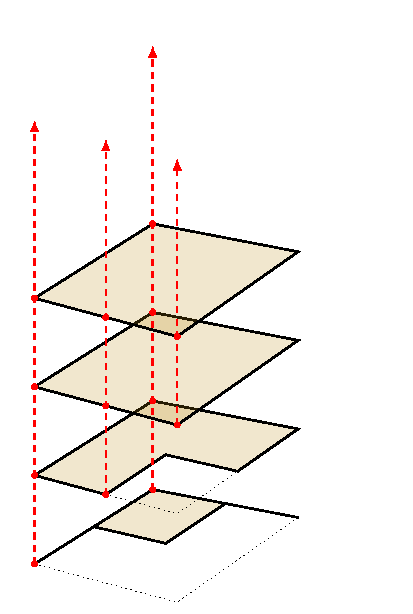
\includegraphics{img/3d_towers_no_text}
\end{figure}

\lipsum[33-35]

\section{Section 2}
\lipsum[36-40]
